\documentclass[runningheads]{paper}

\usepackage{hyperref}   % hyperlinks
\usepackage{graphicx}
\usepackage{algorithm}
\usepackage[noend]{algpseudocode}
\usepackage{multirow}
\usepackage{longtable}

% Used for displaying a sample figure. If possible, figure files should
% be included in EPS format.
%
% If you use the hyperref package, please uncomment the following line
% to display URLs in blue roman font according to Springer's eBook style:
% \renewcommand\UrlFont{\color{blue}\rmfamily}

% ------------------------------------------------------------------------------

\begin{document}
%
\title{Class Scheduling Problem}
%
\author{Cărămidă Iustina-Andreea - 332CA}
%
\institute{Faculty of Automatic Control and Computer Science \\
University Politehnica of Bucharest \\
\email{iustina.caramida@stud.acs.upb.ro}
}
%
\maketitle              % typeset the header of the contribution
%
\begin{abstract}
    With the rapid growth of student enrollment and the expansion of academic 
    offerings in universities and colleges worldwide, the task of scheduling 
    classes within existing timetables and facilities has become increasingly 
    complex. Today, class scheduling requires consideration of multiple factors, 
    including room availability, capacity, instructors' preferences, and more. This problem is considered to be 
    NP-complete and has received some research during the past few years. 
    Several formulations and algorithms have been proposed to solve scheduling
    problems, most of which are based on local search techniques. In this paper, 
    we propose to compare 2 different types of algorithms to solve the class
    scheduling problem: the random restart Hill-Climbing algorithm and the A-Star algorithm.

\keywords{NP-complete \and A Star \and Hill-Climbing \and searching algorithms \and class scheduling.}
\end{abstract}

% ------------------------------------------------------------------------------
\pagebreak
\section{Introduction}
\subsection{Problem Declaration}

\quad The Class Scheduling Problem represents a critical challenge in the field 
of educational operational research.  Universities contend with an ever-growing 
course catalog, necessitating the efficient allocation of a diverse range of 
classes to classrooms with varying capacities. This optimization problem seeks 
to construct a course schedule that adheres to a comprehensive set of university 
constraints while simultaneously maximizing the effective and efficient 
utilization of existing facilities.

The complexity of the Class Scheduling Problem presents a multifaceted challenge due 
to a confluence of factors. First, there is significant variety in the 
number of students enrolled in each course.  Similarly, classroom capacities 
exhibit a wide range of variation. These factors are further compounded by the 
existence of course-specific classroom constraints. Additionally, faculty 
members often express preferences regarding the day of the week, time slot, 
and even break schedule for their assigned courses. These factors, combined 
with the need to satisfy a multitude of university-specific regulations, render 
the task of assigning courses to classrooms a highly intricate endeavor.

Merely ensuring a classroom can accommodate a course's enrolled students is 
insufficient. Such an approach would lead to suboptimal space utilization, 
potentially hindering the educational experience and fostering student 
dissatisfaction. Consider a scenario with two courses: one with six students 
and another with nineteen. Furthermore, imagine two classrooms exist, one 
seating twenty and another seating fifty. While technically feasible to 
schedule either course in either room, a more strategic allocation would be to 
assign the larger course to the larger classroom.

This example exemplifies the multifaceted nature of Class Scheduling Problem. 
Researchers continue to explore sophisticated methods to address this intricate 
problem, with the ultimate goal of ensuring the smooth operation and optimal 
resource allocation within universities.

\subsection{Problem Statement}
\textbf{\textit{Statement:}} Receiving a set of courses, each with a specific
number of students,a set of rooms with a specific capacity, and a list of 
instructors with their list of preferences, the goal is to assign each course to
a room and a time slot, according to a list of constraints.

There are 2 types of constraints that need to be satisfied:
\begin{itemize}
    \item \textbf{Hard constraints:} These constraints must be satisfied in order
    for the solution to be valid. If any of these constraints are not satisfied, 
    the solution is invalid.
    \item \textbf{Soft constraints:} These constraints are not mandatory, but 
    they are taken into account when evaluating the quality of the solution.
\end{itemize}

\subsubsection*{Hard constraints}
\begin{itemize}
    \item Within a designated time slot and in a given room, only one subject may be taught by a single instructor.
    \item During any given time slot, an instructor may teach only one subject, and this instruction must occur within a singular room.
    \item An instructor may conduct classes in a maximum of 7 time slots per week.
    \item Within a specified time slot, a room may accommodate a number of students equal to or less than its predetermined maximum capacity.
    \item All students enrolled in a particular subject must have designated class hours allocated for that subject.
    \item Instructors are restricted to teaching only the subjects in which they are specialized.
    \item All rooms are designated for classes pertaining only to the subjects for which they have been assigned
\end{itemize}

\subsubsection*{Soft constraints}
\begin{itemize}
    \item An instructor may express preferences regarding specific days of the week for teaching or may wish to avoid teaching on certain days.
    \item An instructor may have preferences regarding specific time slots during the day for teaching or may wish to avoid teaching during certain time slots.
    \item An instructor may prefer not to have a break exceeding a certain number of hours between consecutive classes.
\end{itemize}
% 

\subsection{Methods of Approach}
\subsubsection{Random Restart Hill Climbing}
is a local search algorithm commonly applied in optimization 
problems. It begins with an initial solution and iteratively explores 
neighboring solutions, selecting the one that improves the objective function 
the most. This process continues until a local optimum is reached, where no 
better solution can be found in the immediate neighborhood. When the algorithm
reaches a local optimum, it restarts the search from a random initial solution.
The algorithm terminates when a specified number of iterations have been
completed or when a solution that satisfies all constraints is found.

\subsubsection{A Star}
is an informed search algorithm widely used for pathfinding and graph 
traversal tasks. It intelligently combines both actual path costs and heuristic 
estimates to guide the search towards the goal efficiently. A* maintains a 
priority queue of nodes to be explored and selects the most promising node 
based on a combination of the cost incurred so far and the estimated cost to 
reach the goal. This allows A* to efficiently find the optimal path while 
intelligently pruning the search space, making it highly effective for solving 
a wide range of optimization problems.


\subsection{Evaluation}
\quad Both algorithms will be evaluated based on the quality of the solutions they
provide, the time required to find these solutions and the total number of
states explored during the search. The quality of the solutions will be
evaluated based on the number of constraints satisfied.  The time required to 
find the solutions will be measured in milliseconds, and the total number of
states explored will be counted during the search process.

There will be 5 types of tests, describe in \textit{Tests Description} section.

% ------------------------------------------------------------------------------
\section{Algorithm Design}
\subsection{State Representation}

The state representation for the Class Scheduling Problem consists of a
schedule that assigns each course to a room and a time slot. The state is
represented as a class that contains the following fields:
\begin{itemize}
    \item \textbf{file\_name:} The name of the file from which the data was read.
    \item \textbf{yaml\_dict:} A dictionary containing the data read from the file.
    \item \textbf{size:} A tuplet (days, time\_slots) representing the size of the schedule.
    \item \textbf{schedule:} A dictionary that has the following structure: \{(day: str) : \{(time\_slot: (int, int)) : \{(classroom : str) : ((instructor : str), (subject : str))\}\}\}.
    \item \textbf{strudents\_per\_subject:} A dictionary that contains the number of students for each subject that needs to be scheduled.
    \item \textbf{count\_techer\_slots:} A dictionary that contains the number of scheduled slots for each instructor.
    \item \textbf{trade\_off:} A number that represents the trade-off between the number of constraints satisfied and the the choosen classroom at each step (used in A Star).
\end{itemize}

\subsubsection{Initial State}
The initial state is generated as an empty schedule, which is initialized with 
the parameters derived from the input file, including the number of days, time 
slots, and classrooms. Additionally, the number of students per subject is 
obtained from the input file, while the count of scheduled slots for each 
instructor is set to zero.

This initial state serves as the starting point for the search algorithms, 
enabling them to iteratively allocate courses to rooms and time slots until 
a valid schedule is achieved.

An alternative method for generating the initial state involves randomly 
assigning courses, instructors to rooms and time slots in a manner that 
adheres to the hard constraints. A comparative analysis of these two approaches 
will be conducted in the \textit{Initial State Selection} section.

\subsubsection{Generating Neighbors}
The neighbors of a state are generated by considering all possible combinations 
of assigning a course to a room, a time slot and an instructor, while ensuring 
adherence to the hard constraints.

In the initial phase, all potential neighbors that adhere to both the hard and 
soft constraints are generated. Subsequently, in the event that no neighbors 
satisfying all soft constraints are found, a secondary phase ensues where only 
neighbors satisfying the hard constraints are generated. This strategy reduces 
the total number of neighbors generated, allowing the algorithm to prioritize 
those that satisfy all constraints. Consequently, the algorithm minimizes time 
wastage by avoiding the generation of neighbors that would not be utilized, 
resulting in a reduced number of states generated.

\subsubsection{Initial State Selection}
As previously mentioned, the initial state can be generated in two methodologies: either 
as an empty schedule or through the random assignment of courses, instructors, 
and rooms to time slots. The former method exhibits a greater degree of 
determinism, initializing the schedule with vacant slots, whereas the latter 
introduces stochasticity into the initial state generation process.

Upon experimentation with both approaches, it became evident that the random 
initialization method could often yield solutions that fail to adhere to all 
specified soft constraints. This underscores the importance of carefully 
considering all potential subsequent states that may arise from the current 
state when designing the random initialization method.

For instance, in instances where an instructor\'s preferences are violated within 
a particular time slot, the algorithm should endeavor to substitute instructor with 
another whose preferences remain unviolated for that time slot. Moreover, the 
algorithm should endeavor to substitute the time slot with another or substitute
the room with anothers that have the same capacity in total. This approach
was found more difficult to implement. When tring to implement the first two
substitutes, the algorithm was not able to find a solution that satisfies all the
soft constraints and it took quite a lot of time to find a partial solution due to
a large number of constraints that should be checked while creating the neighbors.
On the other hand, this approach will always find a partial solution that 
satisfies all the hard constraints. Thus, this one is recommended in cases 
when the soft constraints are not that important.

The method that I used in 
the end was the empty schedule initialization. It is acknowledged that without 
the random initialization component, the Hill-Climbing algorithm may struggle 
to assign all students to a room, thereby violating a hard constraint. However,
with  the inclusion of the random restart, the algorithm will always find a 
solution that satisfies all the hard constraints, the soft ones being satisfied 
in most of the cases. This approach is recommended in cases when the soft 
constraints are more important than in the previous case and it is easier to 
generate the neighbors.


\subsection{Random Restart Hill Climbing}

As previously mentioned, the Random Restart Hill Climbing algorithm is the 
most suitable for this approach. The algorithm is initialized with an empty
schedule and generates neighbors that adhere to the hard constraints. The
algorithm iteratively explores the neighborhood of the current state, selecting
randomly one of the neighbors that satisfies the most constraints. This process continues until
a local optimum is reached, at which point the algorithm restarts the search.
The algorithm terminates when a solution that
satisfies all constraints is found or when a specified number of iterations / 
restarts have been completed. A pseudocode of the algorithm is presented in Algorithm 1.

\begin{algorithm}
\caption{Random Restart Hill Climbing Algorithm}
\label{alg1}
\begin{algorithmic}[1]
\Procedure{hill\_climbing}{$max\_restarts$} \Return $[is\_final, total\_iters, total\_states, best\_state] $ 
\State $total\_iters = 0$
\State $total\_states = 0$
\State $best\_state = None$

\For{$index$ in $range(max\_restarts)$}
\State $state = InitialState()$
\State $is\_final, iters, states, state = stochastic\_hill\_climbing(state)$
\State $total\_iters += iters$
\State $total\_states += states$

\If{$is\_final$}
\State \Return $[is\_final, total\_iters, total\_states, state]$
\EndIf

\If{$state\ does\ not\ have\ hard\ constraints$}
\If{$best\_state == None$ or $state\ has\ less\ soft\ constraints$
\hspace*{6em}$unsatisfied\ than\ best\_state$}

\State $best\_state = state$
\EndIf
\EndIf
\EndFor

\State \Return $[is\_final, total\_iters, total\_states, best\_state]$

\algstore{bkbreak}
\end{algorithmic}
\end{algorithm}

\addtocounter{algorithm}{-1}
\begin{algorithm}
\caption{Stochastic Hill Climbing}
\begin{algorithmic}[1]
\Procedure{stochastic\_hill\_climbing}{$state, max\__iters$} \Return $[is\_final, total\_iters, total\_states, best\_state] $ 
\State $total\_iters = 0$
\State $total\_states = 0$

\While{$total\_iters < max\_iters$}
\State $total\_iters += 1$

\If{$state\ is\ final$}
\Return $[True, total\_iters, total\_states, state]$
\EndIf

\State $neighbors = state.generate\_neighbors()$
\State $total\_states += len(neighbors)$

\If{$neighbors$ == $None$}
\Return $[False, total\_iters, total\_states, state]$
\EndIf

\State $state = random.choice(from\ neighbors\ one\ of\ the\ neighbors\ with$ \\
\hspace*{2em}$minimum\ number\ of\ constraints\ unsatisfied)$
\EndWhile

\State \Return $[False, total\_iters, total\_states, state]$

\EndProcedure
\end{algorithmic}
\end{algorithm}



\subsection{A Star}
For the A Star algorithm, the state representation is the same as for the Random
Restart Hill Climbing algorithm. The algorithm is initialized with an empty
schedule and generates neighbors that adhere to the hard constraints. The 
algorithm iteratively explores the neighborhood of the current state.

The frontier represents a heap that contains the states that need to be explored.
The diccovered is a dictionary that contains as keys the number of students that
need to be scheduled for each subject and as values the cost of the state that
brought us to this configuration.

The function used in the A Star algorithm is:
\begin{equation}
    f(state) = g(state) + h(state)
\end{equation}

where

\begin{equation}
    h(state) = total\ number\ of\ students\ that\ are\ not\ assigned
\end{equation}
\begin{equation}
    g(state) = number\ of\ constraints\ unsatisfied * weight + trade\_off
\end{equation}
\begin{equation}
    trade\_off = \frac{number\ of\ classrooms(subject)}{total\ number\ of\ classrooms} 
\end{equation}

The heuristic function is admisible, because the return value is always less than
or equal to the actual cost of the state to reach a final one, and is
equal to 0 in the final states. On the other hand, the function h is not consistent,
because a state from discovered can be added to the frontier with a smaller cost.

The cost function is calculated as the number of constraints unsatisfied multiplied
by a weight and the trade off. In cases where the number of constraints unsatisfied
is equal, multiplying it by a weight will prioritize the states that have the trade
off smaller. Moreover, when the number of constraints unsatisfied is different, the
prioritization will be made based on the number of constraints unsatisfied, not on
the trade off.

The trade off is calculated as the number of classrooms that are assigned to a
subject divided by the total number of classrooms. We want to prioritize adding
a subject to a classroom that has fewer subjects assigned to it. For instance,
if we have 2 subjects: A and B, 2 classrooms: 1 and 2, and classroom 1 is assigned
to subject A and classroom 2 is assigned to both subjects, while tring to assign
a subject to classroom 2 we will choose subject B (trade off = 0.5) instead of
subject A (trade off = 1).

The pseudocode of the algorithm is presented in Algorithm 2.

\begin{algorithm} 
\caption{A Star Algorithm}
\label{alg2}
\begin{algorithmic}[1]
\Procedure{astar}{} \Return $[is\_final, total\_iters, total\_states, best\_state] $
\State{$frontier = []$}
\State{$discovered = \{\}$}
\State{$state = InitialState()$}
\State{$frontier.append((f(state), state))$}
\State{$discovered[state] = 0$}
\State{$total\_iters = 0$}
\State{$total\_states = 1$}
\While{$frontier$}
\State{$current\_state = frontier.pop(1)$}
\State{$total\_iters += 1$}
\If{$current\_state\ is_final == 0$}
\Return $[True, total\_iters, total\_states, current\_state]$
\EndIf

\State{$neighbors = current\_state.generate\_neighbors()$}
\State{$total\_states += len(neighbors)$}
\For{$neighbor$ in $neighbors$}
\State{$new\_cost = g(neighbor) + h(neighbor)$}
\State{students\_per\_subject = neighbor.students\_per\_subject}
\If{$students\_per\_subject\ not\ in\ discovered$ or $new\_cost < discovered[students\_per\_subject]$}
\State{$discovered[neighbor] = new\_cost$}
\State{$frontier.append((new\_cost, neighbor))$}
\EndIf
\EndFor
\EndWhile
\State \Return $[False, total\_iters, total\_states, current\_state]$
\EndProcedure
\end{algorithmic}
\end{algorithm}

\subsection{Complexities}
The complexity of the Random Restart Hill Climbing algorithm is $O(n)$, where
$n$ is the total number of iterations. The complexity of the A Star algorithm is
$O(b^d)$, where $b$ is the branching factor and $d$ is the depth of the solution.


The complexity of the generate neighbors function is $O(d*t*c*i*s)$, where $d$ is
the number of days, $t$ is the number of time slots, $c$ is the number of classrooms,
$i$ is the number of instructors and $s$ is the number of subjects. Because the number
of days does not exceed 7 (the worst case) and the number of time slots does not exceed 12, 
the complexity becomes $O(c*i*s)$.

\section{Evaluation}
\subsection{Tests Description}

\subsubsection{orar\_mic\_exact:} Contains 3 courses, 2 rooms, and 13 instructors. The
number of students for each course are 300, 330, and 330. The capacity of the rooms are
20 and 30. The instructors have few preferences.
\subsubsection{orar\_mediu\_relaxat:} Contains 4 courses, 4 rooms, and 18 instructors. The
number of students for each course is 660, 660, 665 and 685. The capacity of the rooms is
25, 25, 35 and 70. The instructors have few preferences.
\subsubsection{orar\_mare\_relaxat:} Contains 8 courses, 6 rooms, and 37 instructors. The
number of students for each course is 470, 475, 475, 495, 500, 530, 535 and 550. The capacity of the rooms is
25, 30, 30, 35, 85 and 85. The instructors have few preferences.
\subsubsection{orar\_constrans\_incalcat:} Contains 4 courses, 2 rooms, and 17 instructors. The
number of students for each course is 720, 750, 780 and 810. The capacity of the rooms is
15 and 90. The instructors have a lot of preferences.
\subsubsection{orar\_bonus\_exact:} Contains 5 courses, 5 rooms, and 23 instructors. The
number of students for each course is 500, 510, 515, 520 and 545. The capacity of the rooms is
15, 15, 15, 15 and 50. The instructors have a lot of preferences, including breaks constraints.

\subsection{Results}
For the Hill-Climbing algorithm, the number of restarts was established at 100,
while the maximum number of iterations for all tests was capped at 1000. In the 
case of the A* algorithm, a weight of 100 was applied.

Each test involved the execution of both algorithms. The ensuing tables depict 
the outcomes across various categories: the count of unsatisfied soft 
constraints, the time taken to attain a solution, the total number of states 
explored during the search, and the iterations needed to reach a solution. 
Additionally, for the Hill Climbing algorithm, the number of restarts executed 
until a solution was obtained is delineated.

The outcomes for the Hill Climbing algorithm are categorized based on the 
number of restarts.

Moreover, the individual results for each test are presented in the following
tables 1 and 2.

\begin{figure}[!]
\centering
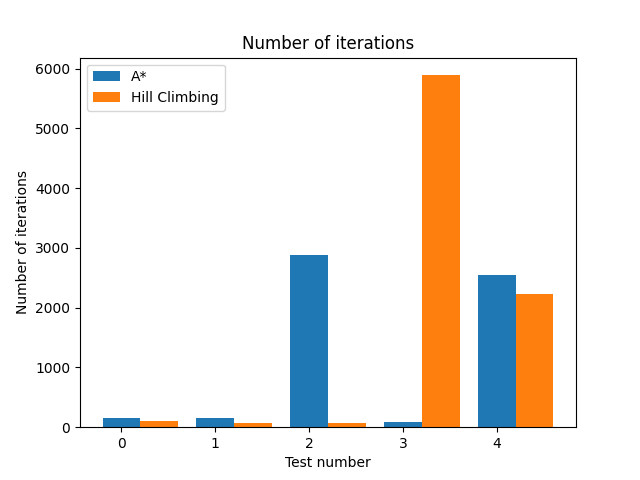
\includegraphics[width=0.8\textwidth]{./images/iterations.png}
\caption{Number of iterations required to find the solution}
\label{fig:empty_graphs}
\end{figure}

\begin{figure}[!]
\centering
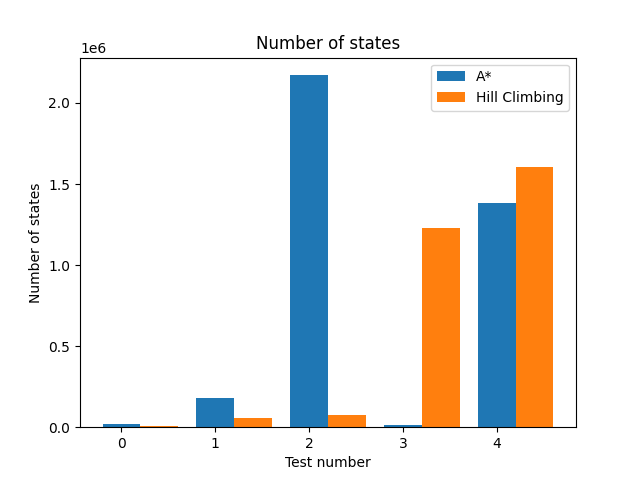
\includegraphics[width=0.8\textwidth]{./images/states.png}
\caption{Total number of states explored during the search}
\label{fig:complete_graphs}
\end{figure}

\begin{figure}[!]
\centering
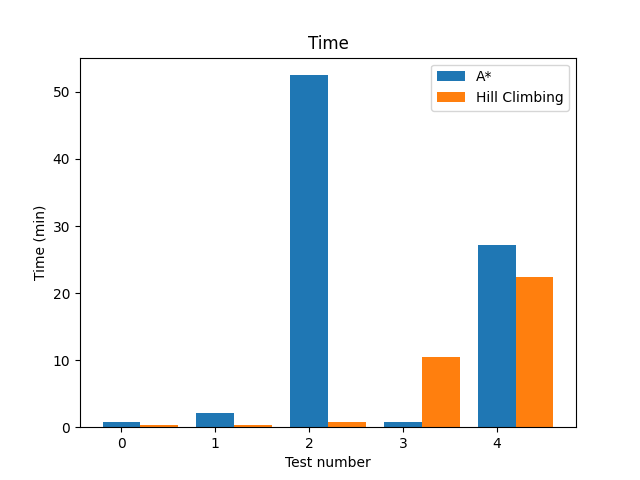
\includegraphics[width=0.8\textwidth]{./images/times.png}
\caption{Time required to find the solution}
\label{fig:bipartite_complete_graphs}
\end{figure}

\begin{figure}[!]
\centering
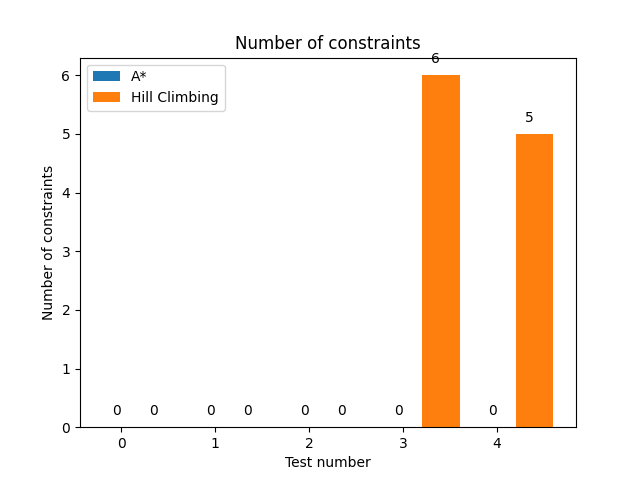
\includegraphics[width=0.8\textwidth]{./images/constraints.png}
\caption{Number of soft constraints unsatisfied}
\label{fig:binary_tree_graphs}
\end{figure}

\begin{figure}[!]
\centering
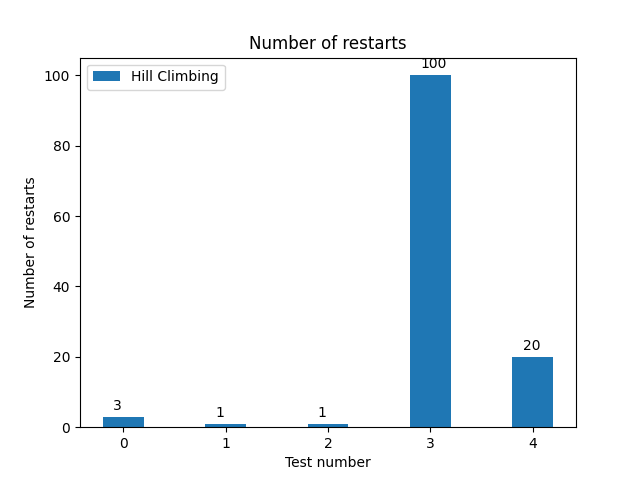
\includegraphics[width=0.8\textwidth]{./images/restarts.png}
\caption{Number of restarts until a solution was found for Hill Climbing}
\label{fig:planar_graphs}
\end{figure}

\begin{table}[!]
\centering
\caption{Results obtained for the Hill Climbing algorithm}
\label{tab:results_hc}
\begin{tabular}{|c|c|c|c|c|c|c|c|}
\hline
\textbf{No. set} & \textbf{No. iterations} & \textbf{No. states} & \textbf{Time mm.ss.ms} & \textbf{No. unsatisfied constraints} & \textbf{No. restars} \\ \hline
\textbf{1} & 106 & 9989 & 0.4.317 & 0 & 3  \\ \hline 
\textbf{2} & 71 & 53875 & 0.34.053 & 0 & 1 \\ \hline
\textbf{3} & 76 & 72621 & 0.77.753 & 0 & 1  \\ \hline 
\textbf{4} & 5889 & 1228027 & 10.40.491 & 6 & 100 \\ \hline 
\textbf{5} & 2221 & 1603927 & 22.47.289 & 5 & 20 \\ \hline 
\end{tabular}
\end{table}

\begin{table}[!]
\centering
\caption{Results obtained for the A Star algorithm}
\label{tab:results_astar}
\begin{tabular}{|c|c|c|c|c|}
\hline
\textbf{No. set} & \textbf{No. iterations} & \textbf{No. states} & \textbf{Time mm.ss.ms} & \textbf{No. unsatisfied constraints} \\ \hline
\textbf{1} & 146 & 17073 & 0.8.537 & 0  \\ \hline
\textbf{2} & 158 & 183159 & 2.12.937 & 0  \\ \hline
\textbf{3} & 2883 & 2171276 & 52.49.856 & 0  \\ \hline
\textbf{4} & 91 & 12368 & 0.8.172 & 0  \\ \hline
\textbf{5} & 2542 & 1385784 & 27.15.878 & 0  \\ \hline
\end{tabular}
\end{table}

\subsection{Observations}

The Hill Climbing algorithm exhibits faster performance compared to the A* 
algorithm primarily due to its local search nature. The Hill Climbing algorithm
is more efficient in terms of the number of iterations required to reach a
solution.

The A* algorithm, while slower, is more effective in terms of the number of
unsatisfied constraints. The A* algorithm consistently yields solutions that
satisfy all constraints, whereas the Hill Climbing algorithm occasionally
encounters unsatisfied constraints.

Recognizing the prolonged duration required to attain a solution for 
orar\_bonus\_exact using the Hill Climbing algorithm, the number of 
restarts was reduced to 20.

The A Star algorithm is more suitable for scenarios similar to orar\_mic\_exact,
orar\_mediu\_relaxat, and orar\_constrans\_incalcat, where the number of
neighbors generated is smaller. In contrast, the Hill Climbing algorithm is
more appropriate for scenarios similar to orar\_mare\_relaxat and orar\_bonus\_exact,
where the number of neighbors generated is larger.

\section{Conclusions}

In summary, within our implementation of the Class Scheduling Problem, 
the Hill Climbing algorithm outperforms the A* algorithm in terms of efficiency.
A* achieves slower solution discovery, but with no unsatisfied constraints. 
Conversely, Hill Climbing is faster, but may occasionally encounter unsatisfied
constraints. The Hill Climbing algorithm is more suitable for scenarios where
the soft constraints are less significant and the time required to find a
solution is a critical factor. In contrast, the A* algorithm is more appropriate
for scenarios where the soft constraints are more significant and the quality of
the solution is paramount.


\pagebreak
% ------------------------------------------------------------------------------

%
% ---- Bibliography ----
%
% BibTeX users should specify bibliography style 'splncs04'.
% References will then be sorted and formatted in the correct style.
%
% \bibliographystyle{splncs04}
% \bibliography{mybibliography}
%
\begin{thebibliography}{8}
    \bibitem{}
    \href{https://en.wikipedia.org/wiki/A*_search_algorithm#Complexity}{A* search algorithm - Wikipedia}
    \bibitem{}
    \href{https://en.wikipedia.org/wiki/Hill_climbing}{Hill Climbing - Wikipedia}
    \bibitem{}
    \href{https://curs.upb.ro/2023/course/view.php?id=13749}{Moodle - Artifical Intelligence Course}
    \bibitem{}
    \href{https://www.researchgate.net/profile/Kian-Pokorny/publication/262277120_Multiple_constraint_satisfaction_problems_using_the_A-star_A_search_algorithm_classroom_scheduling_with_preferences/links/5e57f530299bf1bdb8408b03/Multiple-constraint-satisfaction-problems-using-the-A-star-A-search-algorithm-classroom-scheduling-with-preferences.pdf}{Multiple constraint satisfaction problems using the A-star search algorithm}
    \bibitem{}
    \href{https://d1wqtxts1xzle7.cloudfront.net/68245993/14443-libre.pdf?1626958962=&response-content-disposition=inline%3B+filename%3DCourses_timetabling_based_on_hill_climbi.pdf&Expires=1714507660&Signature=JDd-gaDdE4E7s5P66Op535FyEuysvPoA5o4fcwak4NWT1sQNtVh50ooYa9eSrHu~aHR-Ulabenz910uDjozKpgHivCFkhipTT5bJJL9MensZTSib8TBVzGtBU9lycqCVwilt21Udi0DMgfhERDSgCcR4vO8hmlFlxOLg1exD1fNLE8kxt4S0H2Qfb3nQEHu3kLsicuJNk8wfF~eWpEDUlWsjW9J9IpxuLWP0OICQ7ZReWtx37dHnPN2PTVmFs815NMNi-jyLV0gWWBTAOL7Hn7A5VSg-l~s2e8RAoCjPAYQDRnnznIzOElRy2nTsgkW3mZDzlsntJ3lFur2KquwqNg__&Key-Pair-Id=APKAJLOHF5GGSLRBV4ZA}{Courses timetabling based on hill climbing algorithm}
    
    \end{thebibliography}
\end{document}